%DLC development

\begin{frame}{KASCADE Cosmic-ray Data Center (KCDC)}
    \begin{itemize}
        \small
        \setlength{\itemsep}{0pt}
        \item providing free, unlimited, reliable open access to KASCADE cosmic ray data at \textcolor{blue}{\underline{https://kcdc.ikp.kit.edu}};
        \item almost all KASCADE data is available;
        \item selection of fully calibrated quantities and detector signals;
        \item information platform: physics and experiment backgrounds, tutorials, meta information for data analysis;
        \item archive of KASCADE software and data;
        \item uses modern and open source web technologies.
    \end{itemize}


\includegraphics[height=0.35\textheight]{pics/KCDC-Logo.png}
\hfill
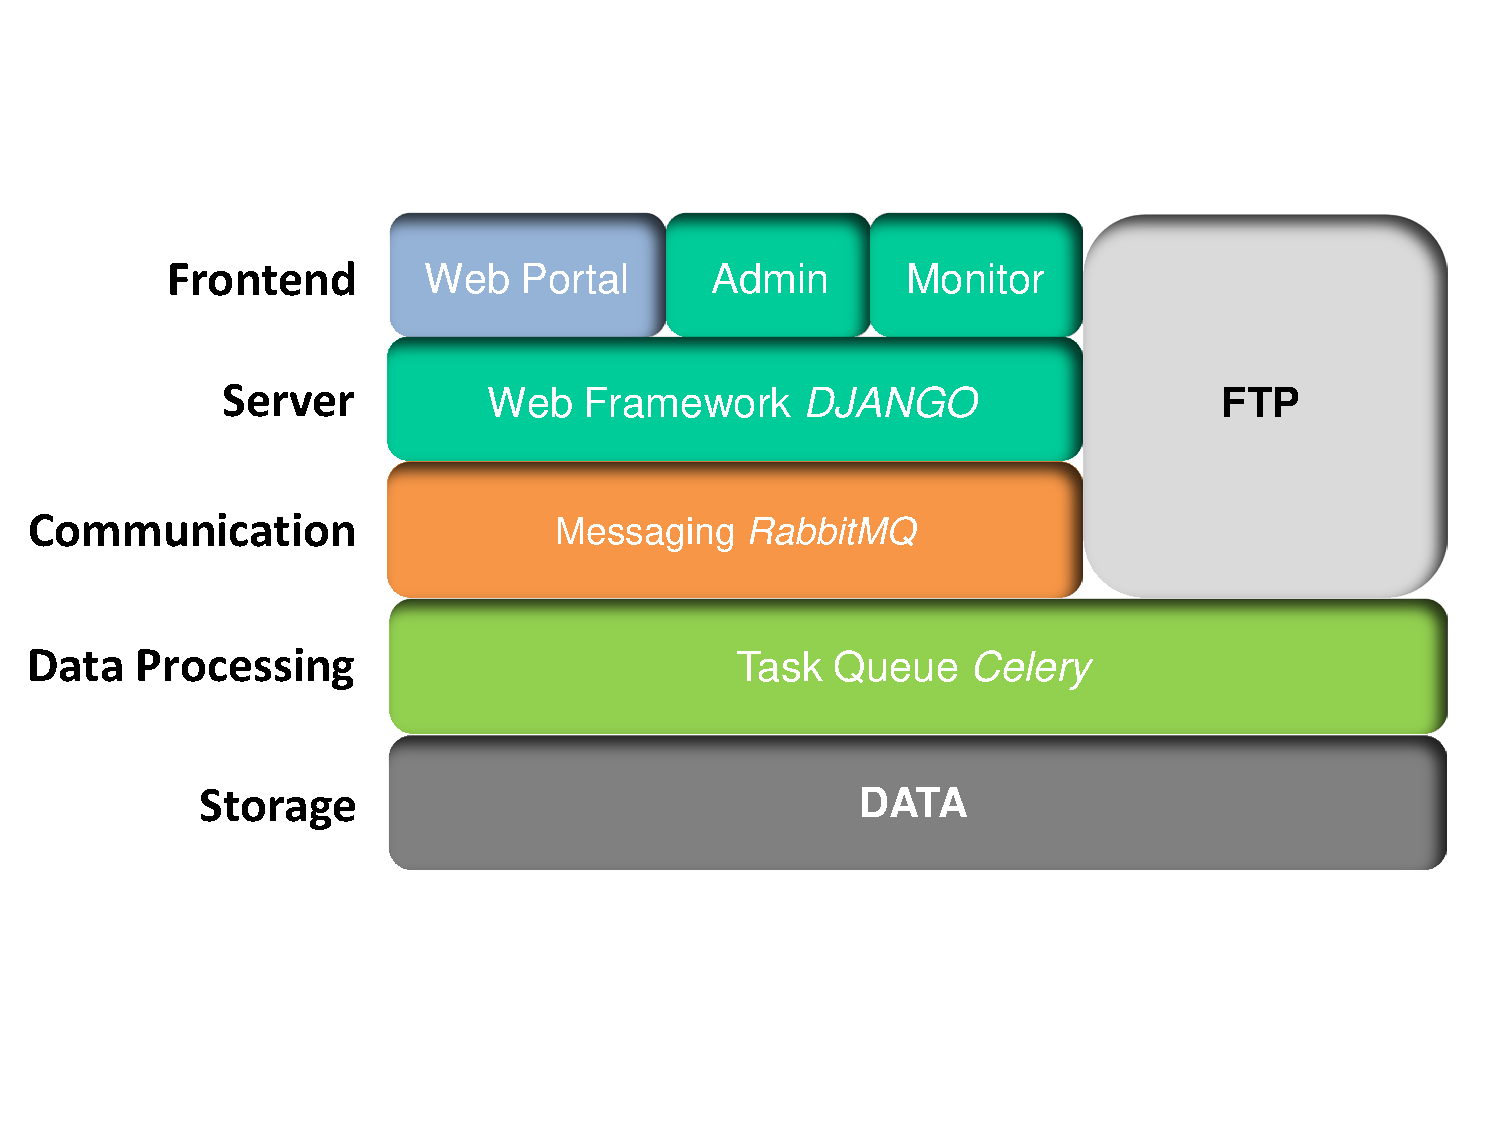
\includegraphics[height=0.35\textheight]{pics/KCDC-IT-Structure.pdf}
\end{frame}

\begin{frame}{TAIGA}
\footnotesize
\vspace{-1em}
\begin{itemize}
 \item Started in the mid 90s, is still operating and continiously enhancend
%  \item Currently consists of 4 detectors presented + TUNKA IACT is under construction;
\end{itemize}
\vspace{-2em}
\begin{minipage}[t]{0.31\textwidth}
  \begin{block}{\small Tunka-133}
    \parbox[c][0.20\textheight][t]{1\textwidth}{
      \centering
      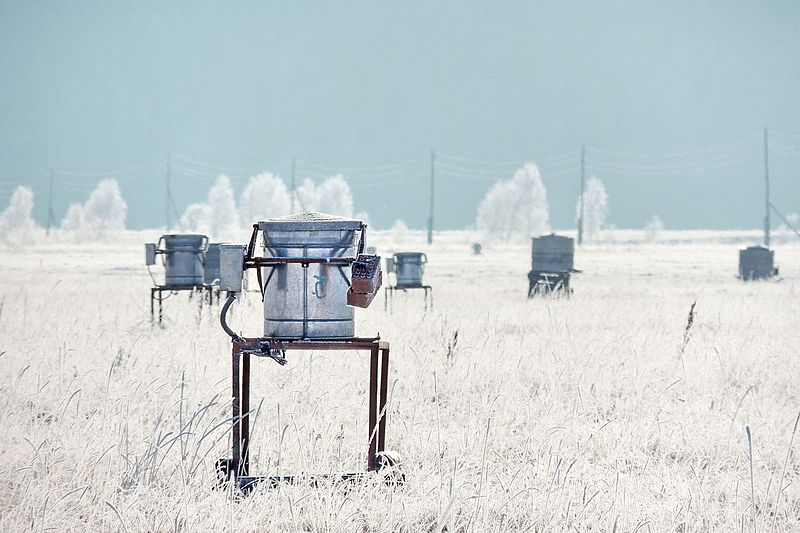
\includegraphics[width=0.7742\textwidth]{pics/Tunka-133.jpg}
    }
    \hfill
    \parbox[c][0.15\textheight][t]{1\textwidth}{
      \begin{itemize}
        \setlength{\itemsep}{0pt}
        \item 133 photomultipliers
        \item measures EAS Cherenkov light
      \end{itemize}
    }
  \end{block}
\end{minipage}
\hfill
\begin{minipage}[t]{0.31\textwidth}
  \begin{block}{\small Tunka-Rex}
    \parbox[c][0.20\textheight][t]{1\textwidth}{
      \centering
      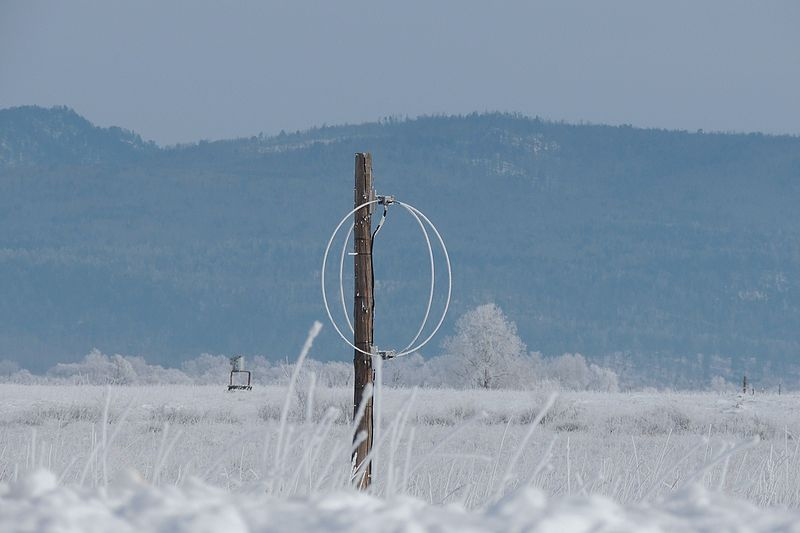
\includegraphics[width=0.7742\textwidth]{pics/Tunka-Rex.jpg}
    }
    \\
    \parbox[c][0.15\textheight][t]{1\textwidth}{
      \begin{itemize}
        \setlength{\itemsep}{0pt}
        \item 63 antennas
        \item measures EAS radio-emission
      \end{itemize}
    }
  \end{block}
\end{minipage}
\hfill
\begin{minipage}[t]{0.31\textwidth}
  \begin{block}{\small Tunka-HiSCORE}
    \parbox[c][0.20\textheight][t]{1\textwidth}{
      \centering
      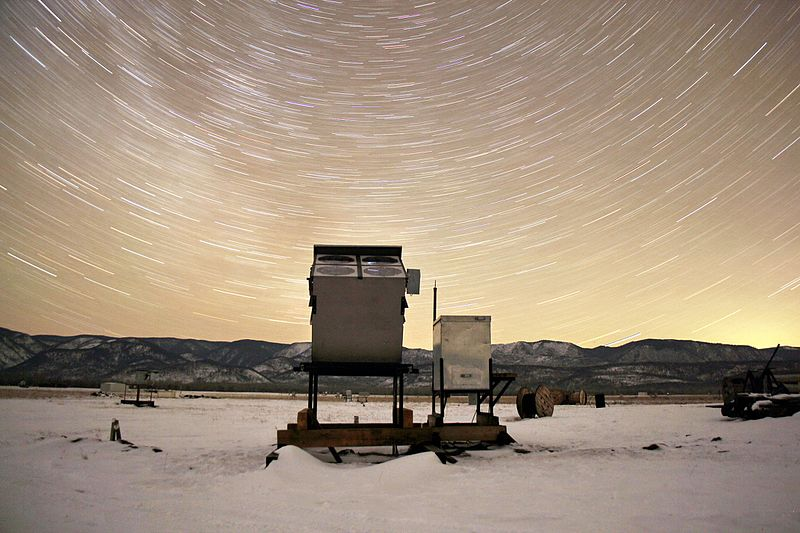
\includegraphics[width=0.7742\textwidth]{pics/Tunka-HiSCORE.jpg}
    }
    \\
    \parbox[c][0.15\textheight][t]{1.1\textwidth}{
      \begin{itemize}
        \setlength{\itemsep}{0pt}
        \item 47$\times$4 photomultipliers
        \item measures EAS Cherenkov light
      \end{itemize}
    }
  \end{block}
\end{minipage}

\vspace{-1ex}
\begin{minipage}[t]{0.48\textwidth}
  \begin{block}{\small Tunka-Grande}
    \parbox[c][0.21\textheight][t]{0.43\textwidth}{
      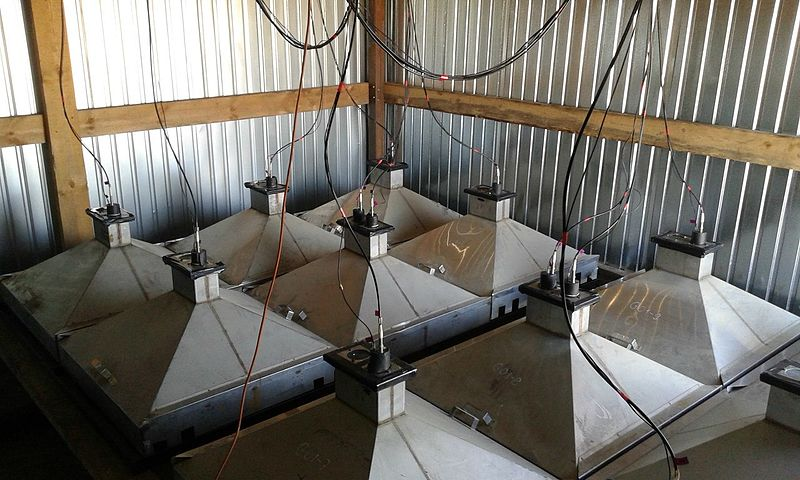
\includegraphics[width=0.50\textwidth]{pics/Hiller_Roman-005.jpg}
    }
    \hfill
    \parbox[c][0.21\textheight][t]{0.55\textwidth}{
      \begin{itemize}
        \setlength{\itemsep}{0pt}
        \item 380 scintillators 0.64m$^2$ each
        \item measures $e$/$\mu$ from EAS
      \end{itemize}
    }
  \end{block}
\end{minipage}
\hfill
\begin{minipage}[t]{0.48\textwidth}
  \begin{block}{\small Tunka-IACT}
    \parbox[c][0.21\textheight][t]{0.43\textwidth}{
      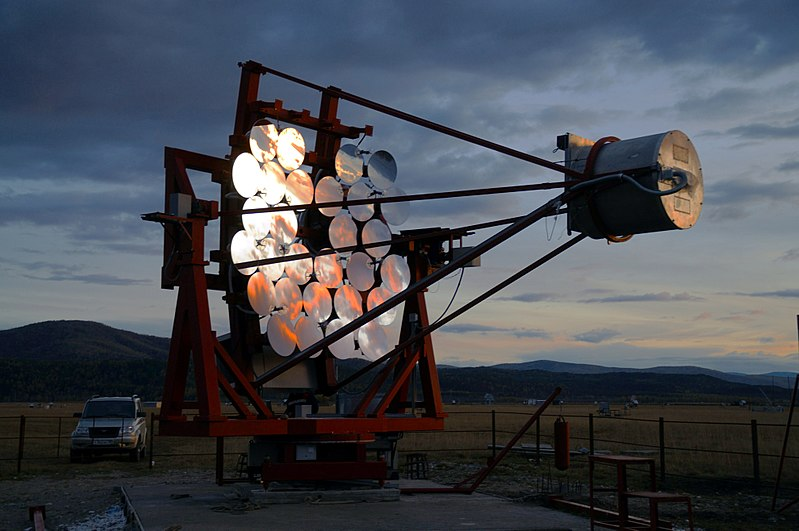
\includegraphics[width=0.50\textwidth]{pics/Tunka-Iact.jpg}
    }
    \hfill
    \parbox[c][0.21\textheight][t]{0.55\textwidth}{
      \begin{itemize}
        \setlength{\itemsep}{0pt}
        \item Imaging Air Cherenkov Telescopes
        \item is being extended
      \end{itemize}
    }
  \end{block}
\end{minipage}
\end{frame}

\begin{frame}{KASCADE and TAIGA data rates}
\begin{minipage}[c]{0.5\textwidth}
  \begin{itemize}
    \item KASCADE:
    \begin{itemize}
      \item 450 000 000 events
      \item $\sim 4$~TB of measured data
    \end{itemize}
    \vspace{2em}
    \item planned TAIGA rate: $\sim 20$~TB/year
    \begin{itemize}
      \item HiSCORE: $\sim 18$~TB/year
      \item IACT: $\sim 1.5$~TB/year
      \item others: $\sim 0.5$~TB/year
    \end{itemize}
  \end{itemize}
\end{minipage}
\hfill
\begin{minipage}[c]{0.49\textwidth}
\vspace{-3.5em}
  \begin{itemize}
    \item current TAIGA rate: 
    \begin{itemize}
      \item $\sim 50$~TB of raw data;
      \item $\sim 8$~TB/year of reconstructed data:
      \begin{itemize}
        \item HiSCORE: $\sim 6.4$~TB/year
        \item IACT: $\sim 1$~TB/year
        \item others: $\sim 0.5$~TB/year
      \end{itemize}
    \end{itemize}
  \end{itemize}
\end{minipage}
\end{frame}

\begin{frame}{DLC Architecture}
\begin{minipage}[c]{0.63\textwidth}
  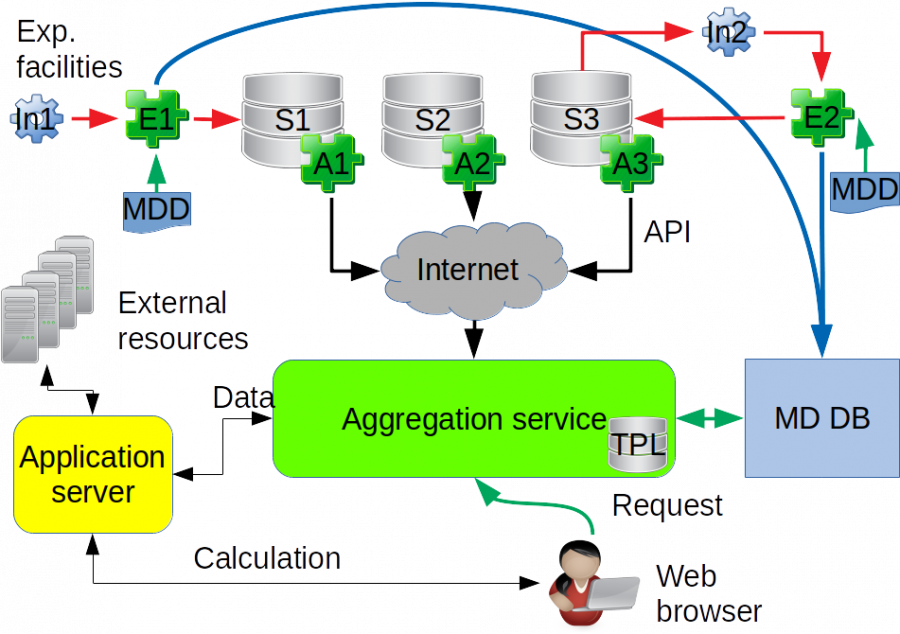
\includegraphics[width=1\textwidth]{pics/arch_appds.png}
\end{minipage}
\hfill
\begin{minipage}[c]{0.33\textwidth}
%   \small
  \textbf{Conceptual features:}
  \begin{itemize}
    \item Plugins for online processing
    \item Fast data search with metadata DB
    \item Data caching on aggregation server
    \item Vispa-like interface
%     \setlength{\itemsep}{0pt}
%     \setlength{\parskip}{0pt}
%     \item\textbf{Si} — local data storages;
%     \item\textbf{Ini} — data sources of different types;
%     \item\textbf{MDD} — metadata description;
%     \item\textbf{Ei} — metadata extractors;
%     \item\textbf{Ai} — adapters, provide API for data access;
%     \item\textbf{TPL} — template library;
%     \item\textbf{MD DB} — metadata database.
  \end{itemize}
\end{minipage}
\end{frame}
